%!TEX encoding = UTF-8 Unicode
\documentclass[12pt]{article}

%\usepackage{eurosym} 
\usepackage{makeidx} 
\usepackage{amsthm,amsmath,amssymb,amsfonts} 
\usepackage{geometry} 
\usepackage{graphics}

%{xltxtra} 
%\synctex=1
\usepackage{tikz} 
\usepackage{xcolor} 
\usepackage{hyperref} 
\usepackage{array}
\usepackage[center]{caption} 
\usepackage{subfig} 
\usepackage{enumerate} 
\usepackage[onehalfspacing]{setspace} 
\usepackage[round]{natbib} 
\usepackage[obeyDraft,colorinlistoftodos]{todonotes}
%to be able to put math in section title without error message: 

\usepackage{pifont}% http://ctan.org/pkg/pifont
\newcommand{\cmark}{\ding{51}}%
\newcommand{\xmark}{\ding{55}}%

\setcounter{MaxMatrixCols}{10}
\usepackage{multirow}

\pagestyle{myheadings} 
\newtheorem{theorem}{Theorem} 
\newtheorem{acknowledgement}{Acknowledgement} 
\newtheorem{algorithm}{Algorithm} 
\newtheorem{assumption}{Assumption} 
\newtheorem{axiom}{Axiom} 
\newtheorem{fact}{Fact} 
\newtheorem{claim}{Claim} 
\newtheorem{conclusion}{Conclusion} 
\newtheorem{condition}{Condition} 
\newtheorem{conjecture}{Conjecture} 
\newtheorem{corollary}{Corollary} 
\newtheorem{criterion}{Criterion} 
\newtheorem{example}{Example} 
\newtheorem{exercise}{Exercise} 
\newtheorem{lemma}{Lemma} 
\newtheorem{proposition}{\text{Pr}oposition} 
\theoremstyle{definition} 
\newtheorem{definition}{Definition} 
\newtheorem{notation}{Notation} 
\newtheorem{problem}{\text{Pr}oblem} 
\theoremstyle{remark} 
\newtheorem{remark}{Remark} 
\newtheorem{solution}{Solution} 
\newtheorem{summary}{Summary} 

% ===============================================================
% = These set new numbering for theorems and lemmas in appendix =
% ===============================================================
\newtheorem{thm}{Theorem}[section] 
\newtheorem{lem}[thm]{Lemma} 
\newtheorem{prop}[thm]{\text{Pr}oposition} 
\newtheorem{cor}[thm]{Corollary}

\onehalfspacing 
%\setlength{ 
%\topmargin}{-.4in} 
%\setlength{ 
%\textheight}{23cm}

\begin{document}

\title{Promises and Communication}
\thanks{The research leading to these results has received funding from the European Research Council under the European Union's Seventh Framework Programme (FP/2007-2013) ERC Grant Agreement n. 339950}
\author{Patrick Legros
\thanks{Universit\'e libre de Bruxelles (ECARES) and C.E.P.R} } 
\date{\today}

\maketitle


\begin{abstract}
	
	\noindent \textbf{Keywords:}\\
	\noindent \textbf{JEL codes:} 
\end{abstract}


Players have basic types $C,D$ with payoffs when there is no communication
\begin{table}
	[!htbp] \centering 
	\begin{tabular}
		{c c c} {\small{Own$\backslash$} Opponent} & $H$ & $L$ \\
		\cline{2-3} $H$ & $a$& $10$\\
		\cline{2-3} $L$ & $24$& $20$ \\
		\cline{2-3}\\
		\multicolumn{3}{c}{Type $C$} 
	\end{tabular}
	\hspace{5em} 
	\begin{tabular}
		{c c c} {\small{Own$\backslash$} Opponent} & $H$ & $L$ \\
		\cline{2-3} $H$ & $22$& $10$\\
		\cline{2-3} $L$ & $24$& $20$ \\
		\cline{2-3}\\
		\multicolumn{3}{c}{Type $D$} 
	\end{tabular}
	\caption{Regime NC ($a\in\{30,50\}$)} 
\label{tbl:NC} \end{table}

For each type, a proportion $\pi$ of players keeps promises while a proportion $1-\pi$ bears a small cost (equal to $1$) from breaking promises. If during a communication phase a message is sent, the understanding is that the player promises to take action $H$ in the continuation game. A type who does not feel bound to promises has same payoffs as in Table \ref{tbl:NC} for the action $H$, and the payoffs minus one for the action $L$; a type who is bound by her promise has a dominant strategy to play $H$ in the continuation game (or faces a large cost-of-lying). This regime is call CT ("cheap talk").

The last regime $F$ is when there is also an exogenous cost of sending messages and we fix this cost at $3$. The difference with the previous regime CT is that a player incurs the cost of $3$ independently of her future actions, while in the CT regime, she incurs the cost-of-lying, of not keeping promises, only if she plays $L$ later on. Hence, the exogenous cost makes it uniformly less appealing to communicate. Note that once the cost of communication is paid, the marginal incentives for playing $H$ versus $L$ are identical to the CT regimes (but all payoffs are decreased by $3$).

%


\section{No-Communication  (NC)} 

% (fold)
\label{sec:no_communication_possible} It is clear that types $D$ players have a dominant strategy to play $L$, and it is sufficient to consider the strategy of types $C$ players, that is the probability $x$ that they play $H$. Because a player has a half-chance of being paired with a $C$ player, playing $H$ yields an expected payoff of $\frac{1}{2}(x a+(1-x)10)+\frac{1}{2}10=10+(a-10)\frac{x}{2}$, while playing $L$ gives an expected payoff of $20+ 2x$. Therefore, the best response of type $C$ is 
\begin{align*}
	BR(x)=
	\begin{cases}
		0 & \text{ if } x < \frac{20}{a-14}\\
		[0,1]&\text{ if } x = \frac{20}{a-14}\\\
		1&\text{ if }x > \frac{20}{a-14}\ 
	\end{cases}
\end{align*}
Clearly, as $a=30$, $\frac{20}{a-14}>1$, and therefore the only equilibrium is for both types to play $L$? However, if $a=50$, there are three equilibria: the two pure strategy profiles $(L,L),(H,L)$ and the mixed strategy profile $(x=5/9,L)$. 
\begin{proposition}\label{prop:nocomm} 
If communication is not possible:
	\begin{enumerate}
		[(i)] 
		\item If $a=30$, the only equilibrium is for both types to play $L$. 
		\item If $a=50$, there are two pure strategy equilibria $(L,L)$ and $(H,L)$, and another equilibrium where types $C$ play $H$ with probability $5/9$ and type $D$ play $L$. 
	\end{enumerate}
\end{proposition}
%
% section no_communication_possible (end)


\section{Communication with Cost-of-Lying (CT)} \label{sec:communication_without_penalties}  In the communication stage, actions are $\{0,1\}$, where $0$ means not sending a message and $1$ sending a message. A strategy for types $C$ is the probability $\alpha$ of sending a message and a strategy for $D$ is the probability $\beta$ of sending a message.

After the communication stage, there can be four states $(i,j)\in\{0,1\}^2$. We use the convention that for a given player $(i,j)$ denotes the action $i$ that the player has taken during communication and the action $j$ that the opponent has taken during communication. Therefore, a player who observes $(i,j)$ knows that the opponent observes $(j,i)$.

There are four possible types of players $C_1,C_\infty,D_1,D_\infty$ where the subscript $1$ indexes a player who has a cost-of-lying of $1$ and the subscript $\infty$ indexes a player who is bound by promises.

Without communication, type $D$ has a dominant strategy to play $L$ in the continuation game. Type $D_\infty$ can, by communicating, commit to play $H$ but the opportunity cost of doing so is to be able to have a higher payoff if he faces a player who plays $H$ by not communicating. By contrast for a $D_1$ type, communication does not bring such a cost but may a-contrario induce the other player to play $H$. Communication is therefore subject to a basic adverse selection problem, as types who do not keep their promises are more likely to be willing to communicate.

Strategies in the communication game are $(\alpha_1,\alpha_\infty,\beta_1,\beta_\infty)$, where $\alpha_k$ is the strategy of $C_k$ and $\beta_k$ is the strategy of $D_k$.

Once a state $(i,j)$ is realized, each player updates his belief about the type of the opponent. For instance, in state $(1,1)$ the posterior that the opponent is type $C_\infty$ is

%
\[ p(C_\infty|1)=\frac{\pi \alpha_\infty}{\pi(\alpha_\infty+\beta_\infty)+(1-\pi)(\alpha_1+\beta_1)}. \]

%
Given these posterior beliefs, players play state-contingent strategies in the continuation game. For $D_1$ and for $D_\infty$ who does not communicate the dominant strategy is $L$, while for $D_\infty$ and $C_\infty$ who communicate the dominant strategy is to play $H$. Finally, for $C_1$ or $C_\infty$ who does not communicate, we assume that they use the same strategy in the continuation game (this is consistent with identifying a `type' with the payoff structure), and we let $x(i,j)$ be the probability that a player facing state $(i,j)$ plays $H$.

Table \ref{tbl:strategies} summarizes this discussion. 
\begin{table}
	[htb!] 
	\centering 
	\begin{tabular}{lllll}
		 
		 \textbf{} & \textbf{$C_1$} & \textbf{$C_\infty$} & \textbf{$D_1$} & \textbf{$D_\infty$}\\
		\hline 
		Message 	& $x(1,j)$ & $H$ 	 	& $L$ 	& $H$\\
		No Message 	& $x(0,j)$ & $x(0,j)$ 	& $L $	& $L$\\
		\hline
	\end{tabular}
	\caption{Strategies ($j\in\{0,1\}$)}
	\label{tbl:strategies}
\end{table}
%
A no-communication outcome is always possible and we will be searching for equilibria in which communication yields more coordination on $H$ than in regime NC. %As will become clear during the proofs, there is no loss of generality in assuming that $x(0,0)=0$: by increasing $x(0,0)$, incentives to communicate are reduced for both types $C$ (who can benefit from coordination on $H$ without having to bear the cost-of-lying) and for types $D$ (who can also avoid the cost-of-lying while deviating to $L$).

\subsection{All Types Communicate}
Communication serves as a commitment device when there is a positive cost-of-lying. For instance types $C_\infty$ and $D_\infty$ are fully committed to play $H$ after sending a message. This commitment by types $C_\infty$ and $D_\infty$ induces also type $C_1$ to play $H$ more often than in the regime NC. However commitment entails a cost if the benefit from coordination on $H$ is small.

Formally, if all types send a message, the posterior beliefs are the same as the prior. Let $x(1,1)$ be the equilibrium action of types $C$ and assume that $x(i,0)=0$ for all $i$ (this gives the most chances to this equilibrium).

By sending a message, a type $D_\infty$ player faces types $C_1$ who will play $H$ with probability $x(1,1)$, types $C_\infty,D_\infty$ who play $H$ with probability $1$ and a type $D_1$ player who will play $L$, therefore her  expected payoff by sending a message is equal to  $10+12\pi+6(1-\pi)x(1,1)$. Hence her maximum payoff from communication  when $x(1,1)=1$ is equal to $16+6\pi$.

By not sending a message, type $D_\infty$ faces types $C_1$ and $D_1$ who play $L$ and types $C_\infty$ and $D_\infty$ who play $H$. Contrary to the previous case, the player can now play $L$. Therefore her expected payoff is $\pi 24+(1-\pi)20=20+4\pi$, which is clearly greater than $16+6\pi$ for any value of $\pi$.

Hence, there is no equilibrium in which all types communicate.


\subsection{A Basic Adverse Selection Problem: Only Types $C$ Communicate} Suppose that types $C$ communicate, while types $D$ do not communicate (it should be clear shortly that if $D_1$ does not communicate, then $D_\infty$ does not communicate either: they both have the same expected payoff by not communicating but type $D_\infty$ has a lower expected payoff than type $D_1$ by communicating since she is constrained in her best-responses). 

For a type $D_1$, playing $L$ in the continuation game is a dominant strategy (if she communicates, while her payoffs if playing $L$ are decreased by $1$, they still dominate the payoffs from playing $H$). Hence, by sending a message $D_1$ has an expected payoff of 
\[
\frac{1}{2}(\pi 24 + (1-\pi)(20+4x(1,1))+\frac{1}{2}(20)-1
\]
while by not sending a message, she has an expected payoff of
\[
\frac{1}{2}(\pi 24 + (1-\pi)(20+4x(1,0))+\frac{1}{2}(20)
\]
and therefore not sending a message is (weakly) optimal for $D_1$ when $	x(1,1)-x(1,0)\leq\frac{1}{2(1-\pi)}$.  
%
In state $(1,0)$, the posterior beliefs of the communicating player is that she faces a type $D$ with probability one. Therefore, a type $C_1$ who communicated but has an expected payoff of $10$ if she plays $H$ an an expected payoff of $20-1$ if she plays $L$. Therefore, she must use $x(1,0)=0$. It follows that the condition for type $D_1$ not to communicate is
%
\begin{equation}\label{cond-IC-D1}
	x(1,1)\leq\frac{1}{2(1-\pi)}.
\end{equation}
%
This condition holds if $\pi\geq \frac{1}{2}$. If $\pi<\frac{1}{2}$, the condition holds only if $x(1,1)<1$, implying that $C_1$ plays a mixed strategy in the continuation game or plays $L$.

\paragraph{Case $x(1,1)=0$.} After communicating type $C_\infty$ faces an opponent who plays $H$ only if that player is of type $C_\infty$. Hence, her expected payoff is equal to $\frac{\pi}{2}a + (1-\frac{1}{2}\pi)10=10+\frac{\pi}{2}(a-10)$. By not communicating, she faces opponents who play the same actions, that is only type $C_\infty$ plays $H$. By not communicating and playing $H$ when the state is $(0,1)$ and playing $L$ when the state is $(0,0)$, $C_\infty$ gets $\frac{1}{2}(\pi a + (1-\pi)) + \frac{1}{2} 20 = 15 + \frac{\pi}{2}(a-10)$ which is larger than $C_\infty$'s expected payoff from communication. A contradiction.

\paragraph{Case $x(1,1)\in (0,1)$.} There are two out-of-equilibrium states for player $C$ (when she deviates by not communicating). If the state is $(0,0)$  the same logic as in state $(1,0)$ implies that $x(0,0)=0$ is optimal. If the state is $(0,1)$  our player believes that she faces a type $C_1$ who is in state $(1,0)$ and plays $L$ and a type $C_\infty$ who plays $H$. Hence, playing $H$ is weakly optimal for types $C_1,C_\infty$ in state $(0,1)$ when $\pi a+(1-\pi)10\geq \pi 24 +(1-\pi)20$, that is when \[x(0,1)>0\Leftrightarrow \pi> \frac{10}{a-14}.\]

We now turn to the other incentive compatibility conditions for players of type $C$.  
Because $x(1,1)\in(0,1)$, a player of type $C_1$ must be indifferent between playing $H$ and $L$ in state $(1,1)$. Because she sent a message, $C_1$ incurs a cost-of-lying of $1$ if she plays $L$ and she is willing to play the mixed strategy when
%
\[
\begin{split}
	\pi a &+(1-\pi)(10+(a-10)x(1,1)) \\
	&=\pi 24 +(1-\pi)(20+4x(1,1)) - 1
\end{split}
\]

or that 
\begin{equation}\label{eq:cond-x11}
	x(1,1)= \frac{9-\pi (a-14)}{(1-\pi)(a-14)}.
\end{equation}
The bound is less than one since $a\geq 23$. It is positive when $\pi\leq \frac{9}{a-14}$, which is smaller than the bound $\frac{10}{a-14}$ for which $x(0,1)$ is positive. Hence, necessarily $x(0,1)=0$.

The bound must be non-negative and smaller than the bound $\frac{1}{2(1-\pi)}$ required for incentive compatibility of type $D_1$, that is we need
\[
\frac{9-\pi (a-14)}{(1-\pi)(a-14)}\leq\frac{1}{2(1-\pi)}.
\]
If $a=30$, the condition holds if $\pi\geq 1/16$; if $a=50$, the condition holds for any $\pi$. Hence a mixed strategy is possible when $a=30$ if $\pi\in[1/16,9/16]$ and when $a=50$ if $\pi\in[0,9/36]$.

What is left to verify is that types $C_k$ prefer to communicate. It is enough to verify that type $C_\infty$ prefers to communicate: a player of type $C_\infty$ has a lower expected payoff from communication than type $C_1$ but the same expected payoff if she does not communicate as type $C_1$.


We consider the two values of $a$.

\underline{If $a=30$,} $C_\infty$'s expected payoff from communication is:
\[
\frac{1}{2}(30 \pi + (1-\pi)(10 + 20 x(1,1)))+\frac{1}{2} 10,
\]
or
\[
10(1+\pi+(1-\pi)x(1,1)).
\] 
If $C_\infty$ does not communicate, she plays $L$ in any state $(0,j)$. Hence her expected payoff is equal to $\frac{1}{2}(20+4\pi)+\frac{1}{2}(20)=20+2\pi$, which is greater than what she obtains under communication for any $\pi$. Hence, it is not possible for only types $C$ to communicate.

\underline{If $a=50$,} From above, communication requires $\pi\leq \frac{9}{36}$. Hence $C_\infty$'s expected payoff from communication is:
\[
\frac{1}{2}(50 \pi + (1-\pi)(10 + 40 x(1,1)))+\frac{1}{2} 10,
\]
or, using $x(1,1)=\frac{9-36\pi}{36(1-\pi)}=\frac{1-4\pi}{4(1-\pi)}$,
\[
10(1+2\pi+2(1-\pi)x(1,1))=15
\] 
which is less than the payoff of $20+2\pi$ and $C_\infty$ does not communicate.

It is therefore not possible to have an equilibrium where only types $C$ communicate and play a mixed strategy in the continuation game.

\paragraph{Case $x(1,1)=1$.} This case is consistent with the incentive compatibility condition for $D_1$ only if $\pi\geq \frac{1}{2}$. 

Player $C_1$ prefers to play $H$ in state $(1,1)$: she gets $a$ by doing so while gets only $23$ by playing $L$.

Turning to the incentives to communicate, we borrow from the previous case, and note that if type $C_\infty$ does not communicate she plays $x(0,1)>0$ only if $\pi\geq \frac{10}{a-14}$. 

\underline{If $a=30$}, and $\pi<\frac{5}{8}$, $x(0,1)=0$ and by not communicating, type $C_\infty$ plays $L$ in all states and therefore has an expected payoff of (only an opponent of type $C_\infty$ plays $H$)  $\frac{\pi}{2}24+\frac{1-\pi}{2}20+\frac{1}{2}20=20+2\pi$. By communicating, she faces a type $C$ with probability $1/2$ and gets $30$ and with probability $1/2$ she faces a type $D$ and gets $10$ (since she plays $H$ against $L$), therefore an expected payoff of $20$, smaller than when she does not communicate.

If $\pi> \frac{5}{8}$, $x(0,1)=1$, and not communicating yields $\frac{\pi}{2}30+\frac{1-\pi}{2}10+\frac{1}{2}20=15+10\pi$. Hence in the region $\pi\geq \frac{1}{2}$, communicating is not a best response for type $C_\infty$ as $\pi\geq\frac{5}{8}$.

\underline{If $a=50$}. Because $\pi\geq \frac{1}{2}>\frac{10}{a-14}$, $x(0,1)=1$. Under communication, player $C_\infty$ gets $50$ against types $C_\infty$ and $C_1$ but only $10$ against the other types, hence an expected payoff of $30$. By not communicating, she gets $50$ against types $C_\infty$ only, $10$ against type $C_1$ (who has state $(1,0)$ and plays $L$) and $20$ against types $D$ (since she faces state $(0,0)$ and plays $L$). Hence her expected payoff under no-communication is $15+20\pi$, which is smaller than $30$ when $\pi\leq \frac{3}{4}$.
%
\begin{proposition}\label{prop:CT-allC}
When there are cost of lying and communication is possible, an equilibrium in which types $C$ communicate and types $D$ do not communicate:
\begin{enumerate}[(i)]
    \item does not exist when $a=30$.
    \item exists when $a=50$ if, and only if $\pi\in\left[\frac{1}{2},\frac{3}{4}\right]$ and $x(1,1)=x(0,1)=1$, $x(0,0)=x(1,0)=0$.
\end{enumerate}
	
\end{proposition}

\begin{remark}
    We have not considered the possibility of mixed strategy in communication. Intuitively, a mixed strategy equilibrium will induce more cooperation the more likely type $C_\infty$ communicates because this type is more committed to play $H$ following communication. However, a simple revealed preference argument suggests that whenever $C_\infty$ is willing to communicate, type $C_1$ is also willing to communicate (remember that the strategic behaviors of types $C_1,C_\infty$ are the same when they do not communicate, but that type $C_\infty$ is more constrained than type $C_1$ in her best-response). Hence, mixed strategies are likely to decreases the level of cooperation conditional on one of the parties communicating. 
\end{remark}

\subsection{Accepting  Adverse Selection: All but $D_\infty$ Communicate} Assume now that types $C$ communicate and that type $D_1$ also communicates. 

In the continuation game, $D_1$ plays $L$ independently of the communication outcome. $D_\infty$ plays $L$ in the equilibrium states $(0,j)$, but plays $H$ in the off equilibrium states $(1,j)$.

In the continuation game, $C_\infty$ plays $H$ in the states $(1,j)$. In state $(1,0)$, $C_1$ believes that she faces a type $D_\infty$ who will play $L$ and therefore plays $L$, or $x(1,0)=0$ (she bears a cost of lying of $1$ but prefers to play $L$ and get $19$ than playing $H$ and get $10$). 

We will first analyze the optimal continuation actions $x(1,1),x(0,1)$ (after the communication phase) and then the incentives of different types to communicate.

\subsubsection*{Continuation Actions}
If $C_k$ does not communicate (off-equilibrium) and the state is $(0,0)$, $C_k$ believes that the other player is type $D_\infty$. As $D_\infty$ plays $L$, $C_k$ will also play $L$ in this case. In the other off-equilibrium state $(0,1)$, $C_k$'s posterior belief is $p(C_1|1)=p(D_1|1)=\frac{1-\pi}{2-\pi}$, $p(C_\infty|1)=\frac{\pi}{2-\pi}$. $C_k$'s expected payoff from playing $H$ is
\[
\frac{1-\pi}{2-\pi} 10 +\frac{\pi}{2-\pi} a + \frac{1-\pi}{2-\pi} 10 = \frac{20+(a-20)\pi}{2-\pi}.
\]
$C_k$'s expected payoff from playing $L$ is
\[
\frac{1-\pi}{2-\pi} 20+\frac{\pi}{2-\pi} 24 + \frac{1-\pi}{2-\pi} 20 = \frac{40-16\pi}{2-\pi}
\]
Therefore, $C_k$ will  play $L$ in state $(0,1)$ when $a=30$ and $\pi \in (0, 10/13)$, plays $H$ if $\pi > 10/13$ and is indifferent when $\pi = 10/13$. When $a=50$,  type $C_k$ plays $L$ if $\pi \in (0, 10/23)$, plays $H$ if $\pi >10/23$ and is indifferent between the two actions when $\pi = 10/23$.

Consider now the possible values of $x(1,1)$ in the continuation game for $C_1$. In the state $(1,1)$, the posterior belief is $p(C_1|1)=p(D_1|1)=\frac{1-\pi}{2-\pi}$, $p(C_\infty|1)=\frac{\pi}{2-\pi}$. The only strategy to determine is that of $C_1$ since, as discussed above, $C_\infty$ plays $H$ after sending a message and type $D_1$ plays $L$.

In state $(1,1)$, $C_1$ playing $H$ dominates playing $L$ when
\begin{align*}
\begin{split}
	\frac{1-\pi}{2-\pi}(10+(a-10)x(1,1))&+\frac{\pi}{2-\pi}(a)+\frac{1-\pi}{2-\pi}(10)\\
	&\geq \frac{1-\pi}{2-\pi}(20+4x(1,1))+\frac{\pi}{2-\pi}(24)+\frac{1-\pi}{2-\pi}(20)-1
\end{split}
\end{align*}
or
\[
\pi\geq \frac{18-(a-14)x(1,1)}{a-5-(a-14)x(1,1)}.
\]
When $a=50$, this condition is equivalent to $x(1,1)\geq \frac{18-45\pi}{36(1-\pi)}=\frac{2-5\pi}{4(1-\pi)}$, and because the right hand side is inferior to one for any $\pi$, it can be optimal for $C_1$ to play $H$. Precisely, either $C_1$ plays the pure strategy $H$ or if $\pi<\frac{2}{5}$ plays the mixed strategy $x(1,1)=\frac{2-5\pi}{4(1-\pi)}$. 

By contrast, the condition when $a=30$ can be satisfied only if  $\pi$ is large enough. Indeed, the condition reduces then to $x(1,1)\geq \frac{18-25\pi}{16(1-\pi)}$, with a right hand side less than one only if $\pi\geq \frac{2}{9}$.

To summarize, players of type $C_1$ play $x(1,1)>0$ in the following cases:
\begin{itemize}
    \item When $a=30$ and $\pi\geq \frac{2}{9}$, in which case either $x(1,1)=1$; or $x(1,1)=\frac{18-25\pi}{16(1-\pi)}$ if $\pi<\frac{18}{25}$.
    \item When $a=30$ and $\pi\leq \frac{2}{9}$, then $x(1,1)=0$.
    \item or when $a=50$, in which case either $x(1,1)=1$; or $x(1,1)=\frac{2-9\pi}{4(1-\pi)}$ if $\pi<\frac{2}{5}$.
\end{itemize}
%
For instance, if $\pi=1/2$,  $C_1$ plays $H$ with probability one if $a=50$ but can play also the mixed strategy $11/16$ if $a=30$. 

\subsubsection*{Incentives to Communicate}
\paragraph{Type $D_\infty$.} By not communicating, a player of type $D_\infty$ has expected payoff of $20+2\pi$ since any opponent plays $L$ in the equilibrium state $(1,0)$ except $C_\infty$ who plays $H$.

By deviating and communicating, $D_\infty$ plays $H$ in the continuation game. She will get $10+12x(1,1)$ if the opponent is $C_1$, $22$ if the opponent is $C_\infty$ and $10$ if the opponent is $D_1$ or $D_\infty$. Hence her expected payoff is equal to $10+6\pi+6x(1,1)(1-\pi)$ which is clearly smaller than $20+2\pi$. Hence $D_\infty$ is incentive compatible.

\paragraph{Type $D_1$.} By not communicating, $D_1$ has also a payoff of $20+2\pi$. In equilibrium $D_1$ communicates, plays $L$ and bears a cost-of-lying. Therefore her expected payoff is equal to $19+2\pi+2x(1,1)(1-\pi)$, which is smaller than $20+2\pi$ when $x(1,1) < \frac{1}{2(1-\pi)}$
the same condition we had in the regime where only types $C$ communicate. This means $D_1$ will communicate only if 
\[
x(1,1)\geq \frac{1}{2(1-\pi)}.
\]
When $\pi>\frac{1}{2}$, then $\frac{1}{2(1-\pi)}>1$ and $D_1$ will not communicate. When $\pi\leq 1/2$, then $\frac{1}{2(1-\pi)}\leq 1$ and $D_1$ can prefer communication if the condition for $x(1,1)$ holds.

When $a=30$, then the mixed strategy $x(1,1)=\frac{18-25\pi}{16(1-\pi)}$ is not greater than $\frac{1}{2(1-\pi)}$ when $\pi\geq \frac{2}{5}$. In this case, $D_1$ will communicate if $x(1,1)=1$. If $\pi\in(0,2/5)$, then both mixed strategy $x(1,1)=\frac{18-25\pi}{16(1-\pi)}$ and $x(1,1)=1$ satisfies the condition and $D_1$ will communicate.

When $a=50$ and $\pi\leq \frac{2}{5}$, the mixed strategy is $x(1,1)=\frac{2-9\pi}{4(1-\pi)}$ which is indeed smaller than $\frac{1}{2(1-\pi)}$. Hence, $D_1$ cannot be incentive compatible with the mixed strategy $x(1,1)=\frac{2-9\pi}{4(1-\pi)}$. If $\pi\in(0, 1/2)$, then $C_1$ can also play a pure strategy $x(1,1)=1$ which is also incentive compatible for $D_1$.

\paragraph{Type $C_\infty$.}  (If this type is incentive compatible, type $C_1$ is also incentive compatible.) If a player of type $C$ does not communicate, her opponent will believe that she is type $D_\infty$. Types $D_k$ and $C_1$ will play $L$, while type $C_\infty$ will play $H$. 

\underline{Case $a=30$.}
As discussed in the analysis of the continuation games, if $\pi<2/9$, $C_1$ plays $L$ in state $(1,1)$ and types $C_k$ also play $L$ in state $(0,j)$. But then, communication is dominated by no communication for players of type $C_\infty$ (they do not change the actions of their opponent by communicating, but are constrained in their best-response).

Hence, $C_\infty$ can be incentive compatible only if $\pi>2/9$. In this case, types $C_1$ play $x(1,1)>0$, but $x(1,0)=0$ and communication modifies the play of such opponents. By communicating a player $C_\infty$ has payoff $\frac{1-\pi}{2}(10+20 x(1,1))+\frac{\pi}{2}30+\frac{1}{2}10$ while by not communicating and playing $L$ her payoff is $\frac{1-\pi}{2}(20+4x(0,1))+\frac{\pi}{2}24+\frac{1}{2}20=20+2\pi + 2 x(0,1)(1-\pi)$. Hence, even if $x(0,1)=0$, communication is best when $x(1,1)>\frac{5-4\pi}{5(1-\pi)}$, which is impossible since the bound is greater than one.

\underline{Case $a=50$.} As mixed strategy in state $(1,1)$ is not incentive compatible for type $D_1$, we will analyse only the case $x(1,1)=1$. In the continuation game, $x(1,1)=1$, and in state $(0,1)$, types $C_k$ play $H$ only if $\pi\geq \frac{10}{23}$. 

(i) Suppose that $\pi> \frac{10}{23}$. 
If $C_\infty$ communicates her expected payoff is $\frac{1-\pi}{2}(10+40x(1,1))+\frac{\pi}{2}50+\frac{1}{2}10=10+20\pi+20(1-\pi)x(1,1)=30$.

Suppose now that $C_\infty$ does not communicate. She can now play $L$ if she faces $D_\infty$, a gain. If she faces an opponent who communicates, she plays $H$ in state $(0,1)$, but faces a more aggressive opponent $C_1$ who plays $L$ instead of $x(1,1)$, a loss. The expected payoff is $\frac{1-\pi}{2}(10)+\frac{\pi}{2}50+\frac{1-\pi}{2}10+\frac{\pi}{2}20=10+25\pi$. It is incentive compatible for player $D_1$ to communicate if $\pi\in(0,1/2)$ and $x(1,1)=1$. Therefore, $C_\infty$'s expected payoff from communication is $30$ and it is larger than her expected payoff from no communication $10+25\pi$ when $\pi\in[10/23,1/2]$.

(ii) Suppose now that $\pi\leq \frac{10}{23}$. If the state is $(0,1)$, type $C_k$ plays $L$. The payoff under no communication is then $20+2\pi$ while the payoff under communication is still $10+20\pi+20(1-\pi)x(1,1)=30$. It is incentive compatible for player $D_1$ to communicate since $\pi\leq \frac{10}{23}<\frac{1}{2}$ and $x(1,1)=1$. The payoff of type $C_\infty$ from communication is $30$ when $x(1,1)=1$, which is always larger than $20+2\pi$.

%
\begin{proposition}\label{prop:CT30-noDinfty}
An equilibrium for which all types except $D_\infty$ communicate:
	\begin{enumerate}[(i)]
		\item does not exist when $a=30$;
		\item does not exist when $a=50$ and $\pi>1/2$;
		\item exists when $a=50$ and $\pi\in[0,1/2]$; in this case the continuation equilibrium entails pure strategies, in particular $x(1,1)=1$ and (out-of-the equilibrium) $x(0,1)=0$ if $\pi\in[0,10/23]$ and $x(0,1)=1$ and (out-of-the equilibrium) $x(0,1)=1$ if $\pi\in(10/23,1/2]$.
	\end{enumerate}
\end{proposition}
%
\subsection{Accepting Adverse Selection: Only Type $C_1$ Communicates}

As discussed in the previous two sections, when $a=30$, there is no equilibrium in which both types $C_1;C_\infty$ communicate. Because types $C_1$ have a lower opportunity cost of communicating (they can play $L$ at cost $1$ if they choose to while $C_\infty$ are committed to playing $H$), we consider now equilibria in which $C_1$ communicates but $C_\infty$ does not communicate.

For such a profile, posterior beliefs in states $(i,1)$  are $p(C_1|1)=1$, $p(t|1)=0$ for $t\neq C_1$, and in states $(i,0)$, $p(C_1|0)=0$, $p(C_\infty|0)=p(D_\infty|0)=\frac{\pi}{1+\pi}$, $p(D_1|0)=\frac{1-\pi}{1+\pi}$.

In the continuation game, type $D_1$ players play $L$ independent of the communication outcome, type $D_\infty$ players play $L$ if the communication outcome is $(0,j)$, while play $H$ in the off equilibrium states $(1,j)$. In the off equilibrium states $(1,j)$, type $C_\infty$ players also play $H$.

In state $(0,0)$, types $C_k$ may be induced to play $H$ if it is likely that they are facing types $C_\infty$. Intuitively, if $x(0,0)$ is positive, it increases the opportunity cost of type $C_1$ to communicate, and we will turn to this later.
\[
\frac{\pi}{1+\pi}(10+(a-10)x(0,0))+\frac{1}{1+\pi}10\geq \frac{\pi}{1+\pi}(20+4x(0,0))+\frac{1}{1+\pi}20, 
\]
hence, $x(0,0)\geq \frac{10}{a-14}\frac{1+\pi}{\pi}$. This is possible only if the bound is less than one, hence if $\pi\geq \frac{10}{a-24}$.
\begin{equation}\label{eq:cond-x00}
    x(0,0)\geq 0 \Leftrightarrow \pi\geq \frac{10}{a-24}
\end{equation}
%

\paragraph{Consider the case $a=30$.} \underline{Continuation strategies:} From \eqref{eq:cond-x00}, when $a=30$ the lower bound is greater than one and therefore $x(0,0)=0$.

In state $(0,1)$, the best response of $C_k$ is to play $H$ when $10+20x(1,0)\geq 20+4x(1,0)$, or when $x(1,0)\geq \frac{5}{8}$.

Consider the continuation best responses of type $C_1$. 

In state $(1,1)$, she plays $H$ as long as $10+20x(1,1)\geq 20+4x(1,1)-1$ or $x(1,1)\geq \frac{9}{16}$. Hence there are two possible Nash equilibria in state $(1,1)$
\begin{equation}\label{BR-11}
	x(1,1)\in\left\{1,\frac{9}{16}\right\}.
\end{equation}

In state $(1,0)$, playing $H$ is a best response if (type $D$ plays $L$ while type $C_\infty$ plays $x(0,1)$):
\[
\frac{\pi}{1+\pi}(10+20 x(0,1))+\frac{1}{1+\pi}10\geq \frac{\pi}{1+\pi}(20+4 x(0,1))+\frac{1}{1+\pi}20 -1,
\]
and the condition will hold in the best case scenario $x(0,1)=1$ when $\pi\geq \frac{9}{7}$ which is clearly not possible. Therefore, $x(1,0)=0$. 

It follows ,that type $C_\infty$ does not play $H$ in the state $(0,1)$. It is also true for off equilibrium state $(0,1)$ for type $C_1$, $x(0,1)=0$. Note that, it is also true that $x(0,0)=0$ for both $C_k$ types.

\underline{Communication incentives:} Given these continuation strategies, a player of type $C_1$ can get the full coordination payoff $a=30$ only if she meets another type $C_1$ and will get $20$ minus the cost-of-lying if she meets another type. Therefore, sending a message is optimal for $C_1$ when $\frac{1-\pi}{2}(10 + 20x(1,1))+\frac{1+\pi}{2}19\geq 20$, that is  
\begin{equation}\label{eq:IC-C1-comm}
C_1\text{ communicates }\Leftrightarrow x(1,1)\geq \frac{1   1-9\pi}{20(1-\pi)},
\end{equation}
%
where the bound is inferior to one when $\pi\in[0,9/11]$ and has value in $\left[\frac{11}{20},1\right]$. Comparing with \eqref{BR-11}, $C_1$ prefers communication if $x(1,1) = 1$ and $\pi\in[0,9/11]$ or $x(1,1) = 9/16$ and $\pi\in[0,1/9]$.

Type $C_\infty$ would be committed to play $H$ if she sends a message and therefore can get $30$ by meeting a $C_1$ type, but $10$ by meeting any other type (including the other players of type $C_\infty$ who are supposed not to send a message in equilibrium). Hence, her expected payoff is $\frac{1-\pi}{2}(10+20x(1,1))+\frac{1+\pi}{2}10=10+10x(1,1) (1-\pi)$ which is strictly less than her expected payoff of $20$ by not sending a message, unless $\pi = 0$ and $x(1,1) = 1$. Hence $C_\infty$ prefers not to send a message.

Consider now the incentive of $D_1$ to send a message. By not sending a message she has an expected payoff of $20$ because $x(1,0)=x(0,1)=x(0,0)=0$. By sending a message she gets $24 x(1,1) + 20(1-x(1,1)) - 1 = 19 + 4x(1,1)$ when meeting a $C_1$ player and $20-1=19$ when meeting other types, so her expected payoff is $\frac{1-\pi}{2}(19 + 4x(1,1))+\frac{1+\pi}{2}19=19+2x(1,1)(1-\pi)$. Hence,
\begin{equation}\label{eq:IC-D1-nocomm}
    D_1 \text{ does not communicate } \Leftrightarrow x(1,1)\leq \frac{1}{2(1-\pi)}.
\end{equation}
%
If $x(1,1)=1$, \eqref{eq:IC-D1-nocomm} is possible only if $\pi\geq \frac{1}{2}$; for the mixed strategy $x(1,1)=\frac{9}{16}$   \eqref{eq:IC-D1-nocomm} requires that $\pi\geq \frac{1}{9}$. Note that, $C_1$ communicates and plays $x(1,1)=1$ when $\pi\in[0,9/11]$ or $x(1,1)=9/16$ when $\pi\in[0,1/9]$

\begin{proposition}\label{prop:CT30-C1}
    When $a=30$, an equilibrium where only $C_1$ communicates exists under the following conditions on the continuation strategies and prior belief $\pi$.
    \begin{enumerate}[(i)]
        \item $x(1,0)=x(0,0)=x(0,1)=0$ 
         \item $x(1,1)=\frac{9}{16}$ if $\pi = \frac{1}{9}$.
         \item $x(1,1) = 1$ if $\pi\in \left[\frac{1}{2}, \frac{9}{11}\right]$
    \end{enumerate}
\end{proposition}

\paragraph{Consider now the case $a=50$.} 
From \eqref{eq:cond-x00}, when $a=50$, it is possible to have $x(0,0)=0$, or $x(0,0)$ positive if  $\pi\geq\frac{5}{13}$, in which case either $x(0,0)=1$ or $x(0,0)=\frac{5}{18}\frac{1+\pi}{\pi}$. 

We consider the cases $x(0,0)=0$ and $x(0,0)>0$ in turn.

\underline{Case $x(0,0)=0$.} In state $(0,1)$, the best response of $C_\infty$ (also for $C_1$ in off equilibrium) is to play $H$ when $10+40x(1,0)\geq 20+4x(1,0)$, or when $x(1,0)\geq \frac{5}{18}$.
%
\begin{equation}\label{eq:x01}
    x(0,1)>0 \Leftrightarrow x(1,0)\geq \frac{5}{18}.
\end{equation}
%
Consider the continuation best responses of type $C_1$. In state $(1,1)$, she plays $H$ as long as $10+40x(1,1)\geq 20+4x(1,1)-1$ or $x(1,1)\geq \frac{1}{4}$. Hence there are two possible (symmetric) continuation equilibria, $x(1,1)=\frac{1}{4}$ and $x(1,1)=1$. 

In state $(1,0)$, playing $H$ is a best response if (type $D$ plays $L$ while type $C_\infty$ plays $x(0,1)$):
\[
\frac{\pi}{1+\pi}(10+40 x(0,1))+\frac{1}{1+\pi}10\geq \frac{\pi}{1+\pi}(20+4 x(0,1))+\frac{1}{1+\pi}20 -1,
\]
that is 
\begin{equation}\label{eq:x10}
    x(1,0)>0 \Leftrightarrow x(0,1)\geq \frac{1+\pi}{4\pi}
\end{equation}
%
Note that \eqref{eq:x01} implies that $x(1,0)>0$ and therefore from \eqref{eq:x10} that $x(0,1)\geq \frac{1+\pi}{4\pi} $, which can happen only if $\pi$ is not smaller than $\frac{1}{3}$. Note also that if $x(0,1)<1$, it must be that $x(1,0)=\frac{5}{18}$ and by \eqref{eq:x10} that $x(0,1)=\frac{1+\pi}{4\pi}$.

\begin{lemma}\label{lem:cont-C1}
The unique continuation strategies when $a=50$ and $x(0,0)=0$ are the following.
\begin{enumerate}[(i)]\setlength\itemsep{-0.1em}
    \item $x(1,1)=1$ or $x(1,1)=\frac{1}{4}$.
    \item $x(0,1)=x(1,0)=0$.
    \item If $\pi\geq \frac{1}{3}$,
    \begin{itemize}
        \item $x(1,0)=x(0,1)=1$
        \item $x(0,1)= \frac{1}{4}\frac{1+\pi}{\pi}$ and $x(1,0)=\frac{5}{18}$.
    \end{itemize}
\end{enumerate}
\end{lemma}
%
We consider the incentive of type $D_1$ to deviate and communicate (which implies that type $D_\infty$ cannot gain either). By not communicating, in state $(0,0)$ the player expects to face opponents who play $L$ and in state $(0,1)$ an opponent of type $C_1$ who plays $x(1,0)$. Hence her expected payoff is 
%
\[
U(D_1):=\frac{1-\pi}{2}(20+4x(1,0))+\frac{1+\pi}{2}20=20+2(1-\pi)x(1,0).
\]
By communicating, type $D_1$ loses $1$ in cost of lying in the continuation game, but the benefit is to ``fool'' $C_1$ and induce her to play $H$ with probability $x(1,1)$, but also type $C_\infty$ who will play $H$ with probability $x(0,1)$. Type $D_1$ player's expected payoff from communicating is then $\frac{1-\pi}{2}(20+4x(1,1))+\frac{\pi}{2}(20+4x(0,1))+\frac{1}{2}20 -1$, or
\[
\hat U(D_1):=19+2(1-\pi)x(1,1)+2\pi x(0,1).
\]
Hence, incentive compatibility $U(D_1)\geq \hat U(D_1)$ requires that 
\begin{equation}\label{eq:IC-D1}
    (1-\pi)(x(1,1)-x(1,0))+\pi x(0,1)\leq \frac{1}{2}
\end{equation}
%
We consider the three cases of Lemma \ref{lem:cont-C1}.
\begin{itemize}
    \item If $x(0,1)=x(1,0)=0$ the condition reduces to $x(1,1)\leq \frac{1}{2(1-\pi)}$. If $x(1,1)=1$, it must be that $\pi\geq \frac{1}{2}$. The mixed strategy $x(1,1)=\frac{1}{4}$ is possible for any value of $\pi$. 
    
    $C_1$ must prefer to communicate. $C_1$'s expected payoff from no communication is $20$, as her opponent will play $L$ in this case. $C_1$'s expected payoff from communication and playing $H$ if the state is (1,1) and $L$ otherwise is $\frac{1-\pi}{2}(10+40x(1,1))+\frac{\pi}{2}(20-1)+\frac{1}{2}(20-1)=\frac{29}{2}+\frac{9}{2}\pi+20x(1,1)(1-\pi)$. When $x(1,1)=1/4$ then $C_1$ will not communicate, but when $x(1,1)=1$ then $C_1$ will communicate if $\pi\leq \frac{29}{31}$. So, in this case, the equilibrium can exist when $\pi\in\left[\frac{1}{2},\frac{29}{31}\right]$ and $x(1,1)=1$.
    
Finally,  $C_\infty$'s must prefer not to communicate. $C_\infty$'s expected payoff from no communication is the same as $C_1$ and equals to $20$. $C_\infty$'s expected payoff from communication is $\frac{1-\pi}{2}(10+40x(1,1))+\frac{\pi}{2}10+\frac{1}{2}(10)=10+20x(1,1)(1-\pi)$. When $\pi\geq 1/2$ then $C_\infty$ prefers no communication.
    
\item $\pi\geq \frac{1}{3}$ and $x(1,0)=x(0,1)=1$. Because $C_1$ and $C_\infty$ use the same strategy after communication (they both weakly prefer to play $H$ in all states) and also when they do not communicate, they must have the same expected payoffs. This means, both types have to be indifferent between communication and no communication, as they cannot have opposite incentives. Type $C_k$'s expected payoff from communication and playing $H$ in states $(1,1)$ and $(1,0)$ is $\frac{\pi}{2}50 + \frac{\pi}{2}(10+40x(1,1))+\frac{1}{2}10= 10+20\pi+20x(1,1) (1-\pi)$. Type $C_k$'s payoff from no communication and playing $H$ in state $(0,1)$ and $L$ in state $(0,0)$ is $\frac{1-\pi}{2} 50 + \frac{1+\pi}{2} 20 = 35-15\pi$. If $x(1,1)=1$, then type $C_k$ is indifferent between communication and no communication if $x(1,1)=1$ and $\pi = 1/3$ or $x(1,1)=1/4$ and $\pi=2/3$. Note that, both cases are consistent with $D_1$'s incentive for not communicating. If $x(1,1)=1$, $D_1$ does not want communication if $\pi\leq 1/2$ and if $x(1,1)=1/4$, $D_1$ does not want communication if $\pi\leq 5/7$.

\item Similar to the previous case, $\pi\geq \frac{1}{3}$ and $x(0,1)=\frac{1+\pi}{4\pi}, x(1,0)=\frac{5}{18}$ requires that both $C$ types have to be indifferent between communication and no communication. Because $C_1$ and $C_\infty$ use the same strategy after communication (they both weakly prefer to play $H$ in all states) and also when they do not communicate, they must have the same expected payoffs. Type $C_k$'s expected payoff from communication and playing $H$ in states\footnote{As $C_1$ is indifferent to play $H$ or $L$ in the state $(1,0)$, we can assume that she plays $H$.} $(1,1)$ and $(1,0)$ is $\frac{1-\pi}{2}(10+40x(0,1)) + \frac{\pi}{2}(10+40x(1,1))+\frac{1}{2}10= 15+5\pi+20x(1,1) (1-\pi)$. Type $C_k$'s payoff from no communication and playing $H$ in state $(0,1)$\footnote{As $C_1$ is indifferent to play $H$ or $L$ in the state $(1,0)$, we can assume that she plays $H$.} and $L$ in state $(0,0)$ is $\frac{1-\pi}{2} (10+40x(1,0)) + \frac{1+\pi}{2} 20 = \frac{5}{9}(37-\pi)$. If $x(1,1)=1$, then type $C_k$ is indifferent between communication and no communication if $x(1,1)=1$ and $\pi = 1$ or $x(1,1)=1/4$ and $\pi=1$. Note that, \textbf{none} of these cases are consistent with $D_1$'s incentive for not communicating. If $x(1,1)=1$, $D_1$ does not want communication if $\pi\leq 1/2$ and if $x(1,1)=1/4$, $D_1$ does not want communication if $\pi\leq 5/7$.
\end{itemize}

\underline{Case $x(0,0)>0$ (and $\pi\geq 5/13$).} Note that type $C_k$ players' incentives in $(1,0)$, $(0,1)$ and $(1,1)$ states are the same as in the case $x(0,0)=0$ described above and we have to check the incentives of the players to communicate. We analyse the three different cases of Lemma \ref{lem:cont-C1}. 

\begin{itemize}
    \item If $x(0,1)=x(1,0)=0$. If $D_1$ communicates and plays $L$ she gets $\frac{1-\pi}{2}(20 + 4x(1,1))+\frac{\pi}{2}20+\frac{1}{2}20-1= 19 + 2x(1,1)(1-\pi)$. If $D_1$ does not communicate and plays $L$ she gets $\frac{1-\pi}{2}(20)+\frac{\pi}{2}(20 + 4x(0,0))+\frac{1}{2}20= 20 + 2x(0,0)\pi$. Not communicating is best when $x(1,1)=1/4$. When $x(1,1)=1$, not communicating is best only if $x(0,0)\geq \frac{1-2\pi}{2\pi}$, which is possible because by assumption $\pi\geq \frac{5}{13}$ implies that  $\frac{1-2\pi}{2\pi}\leq 1$. Note that both the pure strategy $x(0,0)=1$ and the mixed strategy $x(0,0)=\frac{5(1+\pi)}{18\pi}$ satisfy this condition.
    
   $C_1$'s expected payoff from communication and playing $H$ in the state $(1,1)$ and $L$ in the state $(1,0)$ is $\frac{1-\pi}{2}(10+40x(1,1))+\frac{\pi}{2}19+\frac{1}{2}19$. If $C_1$ does not communicate, her expected payoff from playing $H$ in the state $(0,0)$\footnote{As $x(0,0)>0$ then type $C_1$ at least weekly prefers $H$ over $L$.} and $L$ in the state $(0,1)$ is $\frac{1-\pi}{2}20+\frac{\pi}{2}(10+40x(0,0))+\frac{1}{2}10$. If $x(1,1)=\frac{1}{4}$, then $C_1$ communicates if $x(0,0)\leq \frac{9(1+\pi)}{40\pi}$, but as $x(0,0)\in\left\{ 1, \frac{5(1+\pi)}{18\pi} \right\}$ and $\pi\geq 5/13$ this condition never holds. If $x(1,1)=1$, then $C_1$ communicates if $x(0,0)\leq \frac{39-21\pi}{40\pi}$. This condition is satisfied for $x(0,0)=1$ when $\pi\in\left[ \frac{5}{13},\frac{39}{61} \right]$, and is satisfied for $x(0,0)=\frac{5(1+\pi)}{18\pi}$ when $\pi\in \left[ \frac{5}{13}, \frac{251}{289} \right]$. 
    
    Finally, we have to check $C_\infty$'s does not have incentives to communicate. $C_\infty$'s expected payoff from no communication is the same as $C_1$'s payoff from no communication and is given as $\frac{1-\pi}{2}20+\frac{\pi}{2}(10+40x(0,0))+\frac{1}{2}10=15-5\pi+20x(0,0)\pi$. $C_\infty$'s expected payoff from communication is $\frac{1-\pi}{2}(10+40x(1,1))+\frac{\pi}{2}10+\frac{1}{2}10=10+20(1-\pi)x(1,1)$. Hence $C_\infty$ does not communicate when
    $$x(0,0)\geq \left(x(1,1)-\frac{1}{4}\right)\frac{1-\pi}{\pi}$$
   Clearly, the condition holds when $x(1,1)=\frac{1}{4}$ but as we have seen, the mixed strategy is incompatible with $C_1$ communicating.
    
    When $x(1,1)=1$, the condition is $x(0,0)\geq \frac{3}{4}\frac{1-\pi}{\pi}$. The pure strategy $x(0,0)=1$ satisfies the condition only if  $\pi\geq \frac{3}{7}$. The mixed strategy $x(0,0)=\frac{5(1+\pi)}{18\pi}$ satisfies the condition if $\pi\geq \frac{17}{37}$.
    
    Therefore, incentive compatibility is satisfied only if $x(1,1)=1$ and  either
    \begin{itemize}
        \item $x(0,0)=1$ and $\pi\in\left[ \frac{3}{7},\frac{39}{61} \right]$
        \item or $x(0,0)=\frac{5(1+\pi)}{18\pi}$ and $\pi\in \left[ \frac{17}{37}, \frac{251}{289} \right]$.
    \end{itemize}
    The last two cases correspond to $x(1,0)x(0,1)>0$, which is possible when $\pi\geq \frac{5}{13}$ by Lemma \ref{lem:cont-C1}.
    
    \item Case $x(1,0)=x(0,1)=1$. Types $C_1$ plays $H$ in all states after communication, hence has the same expected payoff as a type $C_\infty$ who deviates and communicates. When not communicating, types $C_1,C_\infty$ have the same best responses and expected payoffs. therefore, they must both be indifferent between communicating and not communicating (and using $H$ as a continuation strategy) 
    \[
\frac{1-\pi}{2}(10+40x(1,1))+\frac{\pi}{2}(50)+\frac{1}{2}10=\frac{1-\pi}{2}(50)+\frac{\pi}{2}(10+40x(0,0))+\frac{1}{2}10,
\]
and 
\[
x(0,0)=x(1,1)\frac{1-\pi}{\pi}+\frac{2\pi-1}{\pi}.
\]
If $x(1,1)=1$, $x(0,0)=1$ for all $\pi$. If $x(1,1)=\frac{1}{4}$, $x(0,0)=\frac{7\pi-3}{4\pi}$ which is consistent with $x(0,0)\in\left\{1,\frac{5(1+\pi)}{18\pi}\right\}$, either when $\pi=1$ (for the pure strategy) or $\pi=\frac{37}{53}$ (for the mixed strategy), in which case $x(0,0)=\frac{25}{37}$.

 Hence we can have $x(1,0)=x(0,1)=x(1,1)=1$ in the following cases
\begin{itemize}
    \item $\pi\geq \frac{5}{13}$, and $x(0,0)=x(1,1)=1$,
    \item $\pi=1$, $x(1,1)=\frac{1}{4}$, $x(0,0)=1$
    \item $\pi=\frac{37}{53}$, $x(1,1)=\frac{1}{4}$ $x(0,0)=\frac{25}{37}$.
\end{itemize}

Now we have to check $D_1$'s incentive to communicate. 
    \[
\frac{1-\pi}{2}(24)+\frac{\pi}{2}(20+4x(0,0))+\frac{1}{2}20\geq\frac{1-\pi}{2}(20+4x(1,1))+\frac{\pi}{2}(24)+\frac{1}{2}20-1,
\]
and 
\[
x(0,0)\geq \frac{1}{2\pi} (2x(1,1)(1-\pi) - 3 + 4\pi).
\]

This condition holds for all the three equilibrium candidates above.

\item Case $x(0,1)=\frac{1+\pi}{4\pi},x(1,0)=\frac{5}{18}$. Using the same argument as in the previous case, $C_1,C_\infty$ must be indifferent between communication and no communication. The condition is now,
\[
\frac{1-\pi}{2}(10+40x(1,1))+\frac{\pi}{2}(10+40 x(0,1))+\frac{1}{2}10=\frac{1-\pi}{2}(10+40x(1,0))+\frac{\pi}{2}(10+40x(0,0))+\frac{1}{2}10
\]
or, using the values for $x(0,1),x(1,0)$
\[
x(0,0)=x(1,1)\frac{1-\pi}{\pi}+\frac{19\pi -1}{36 \pi}.
\]
If $x(1,1)=1$, $x(0,0)=\frac{35-17\pi}{36\pi}$, which is consistent with $x(0,0)=1$ only if $\pi=\frac{35}{53}$. It is  consistent with $x(0,0)=\frac{5(1+\pi)}{18\pi}$ only if $\pi=\frac{25}{27}$.

If $x(1,1)=\frac{1}{4}$, $x(0,0)=\frac{4+5\pi}{18\pi}$. This is consistent with $x(0,0)=1$ when $\pi=\frac{4}{13}$, a contradiction to the condition that $\pi\geq \frac{5}{13}$. It is clearly inconsistent  with $x(0,0)=\frac{5(1+\pi)}{18\pi}$. 

Hence, we can have  the mixed strategies in states $(1,0),(0,1)$ only in the following cases.
\begin{itemize}
    \item $\pi=\frac{35}{53}$, $x(1,1)=x(0,0)=1$
    \item $\pi=\frac{25}{27}$, $x(1,1)=1$, $x(0,0)=\frac{26}{45}$.
\end{itemize}
\end{itemize}

Now we have to check $D_1$'s incentive to communicate.
\[
\frac{1-\pi}{2}(20+4x(1,0))+\frac{\pi}{2}(20+4x(0,0))+\frac{1}{2}20\geq \frac{1-\pi}{2}(20+4x(1,1))+\frac{\pi}{2}(20+4 x(0,1))+\frac{1}{2}20-1.
\]
This condition is satisfied for the two equilibrium candidates above.

%
\begin{proposition}\label{prop:CT50-C1}
When $a=50$, an equilibrium where only $C_1$ communicates exists under the following conditions on the continuation strategies and prior belief $\pi$.
	\begin{enumerate}[(a)]
		\item If $\pi\in \left[ \frac{1}{2}, \frac{29}{31} \right]$, $x(0,0)=x(0,1)=x(1,0)=0$ and $x(1,1)=1$.
			
		\item If $\pi\in \left[ \frac{3}{7}, \frac{39}{61} \right]$, $x(0,1)=x(1,0)=0$ and $x(1,1)=x(0,0)=1$.
		
		\item If $\pi\in \left[ \frac{17}{37}, \frac{251}{289} \right]$, $x(0,1)=x(1,0)=0$, $x(0,0)=\frac{5(1+\pi)}{18\pi}$ and $x(1,1)=1$.
		\item If $\pi\in\left[\frac{5}{13},1\right]$, $x(0,1)=x(1,0)=x(1,1)=x(0,0)=1$.
		\item $\pi=\frac{35}{53}$, $x(1,0)=\frac{22}{35}$, $x(0,1)=\frac{5}{18}$, $x(1,1)=x(0,0)=1$
		\item $\pi=\frac{25}{27}$, $x(1,0)=\frac{13}{25}$, $x(0,1)=\frac{5}{18}$, $x(1,1)=1$,  $x(0,0)=\frac{26}{45}$.
		\item $\pi=1$, $x(0,1)=x(1,0)=x(0,0)=1$, $x(1,1)=\frac{1}{4}$.
		\item $\pi=\frac{37}{53}$, $x(0,1)=x(1,0)=1$, $x(1,1)=\frac{1}{4}$, $x(0,0)=\frac{25}{37}$.
		\end{enumerate}
\end{proposition}

The table below contrasts the different ``generic'' equilibrium outcomes (that is when the equilibrium behavior exists for a non-empty interval of $\pi$) in under the three regimes of communication under cheap talk.

\renewcommand{\arraystretch}{1.3}
\begin{table}[!h]
	
\begin{center}
	\begin{tabular}{l|l |l |l}
		
	 %\hline
	 &\multicolumn{3}{c}{Who Communicates}\\
	 & \multicolumn{1}{c}{\bfseries $C_1,C_\infty,D_1$} & \multicolumn{1}{c}{\bfseries $C_1,C_\infty$ } & \multicolumn{1}{c}{\bfseries $C_1$} \\ \hline
	\multirow{3}{*}{$a=30$} & n.a. & n.a. & 
		$x(i,j)=0, (i,j)\neq (1,1)$ \\
		&&& (a) $x(1,1)=\frac{9}{16}$ if $\pi = \frac{1}{9}$ \\
		&&& (b) $x(1,1)=1$ if $\pi\in \left[ \frac{1}{2},\frac{9}{11} \right]$\\
	 \hline
	 \multirow{7}{*}{$a=50$} & (a) $x(i,j)=0, (i,j)\neq(1,1)$	&  $x(0,0)=x(1,0)=0$ & (a) $x(i,j)=0, (i,j)\neq(1,1)$\\
		& $x(1,1)=1$ if $\pi \in \left[0,\frac{10}{23}\right]$ & $x(1,1)=x(0,1)=1$ & $x(1,1)=1$,  $\pi\in \left[ \frac{1}{2}, \frac{29}{31} \right]$ \\
		&(b) $x(0,0)=x(1,0)=0$ & $\pi\in \left[ \frac{1}{2}, \frac{3}{4} \right]$ & (b) $x(1,0)=x(0,1)=0$ \\
		&$x(0,1)=x(1,1)=1$ && $x(1,1)=x(0,0)= 1$, $\pi\in \left[ \frac{3}{7}, \frac{39}{61} \right]$ \\
		& if $\pi\in\left[\frac{10}{23},\frac{1}{2}\right]$ && (c) $x(0,0)=\frac{5(1+\pi)}{18\pi}$, $x(1,0)=$\\
			&&& $x(0,1)=0,x(1,1)=1$, $\pi\in \left[ \frac{17}{37}, \frac{251}{289} \right]$\\	&&& $(d) \pi\in \left[ \frac{5}{13}, 1 \right]$, $x(i,j)=1$\\
	 \hline
	\end{tabular}
	\end{center}
\caption{Cheap Talk Equilibria}
\end{table}

\section{Exogenous Cost of Communication (F)} \label{sec:exogenous_cost_of_communication} 
% (fold)
We introduce now the exogenous cost (equal to $3$) of sending messages. The exogenous cost is sunk once players choose their actions and therefore the set of continuation equilibria is the same as in regime CT.

There are two opposite forces generated by an exogenous cost of communication. First, as in \cite{Spence1973} credible signalling is facilitated. Indeed, types $D$ pay $3$ to communicate but can gain at most $2$ when facing an opponent of type $C$ who plays $H$, while types $C$ can gain more than $3$ when $a$ is large by communicating and inducing cooperation. But because communication is costly, types $C$ players may be reluctant to engage in communication. 

Hence, there can be only two types of equilibria: when both $C_1,C_\infty$ communicate and when only $C_1$ communicates. Compared to our analysis in section \ref{sec:communication_without_penalties} we can ignore the incentive compatibility constraint for communication by $D_1$, that $x(1,1)\leq \frac{1}{2(1-\pi)}$. Because the cost of communication is sunk, the \emph{equilibrium} continuation equilibria are identical to what we derived in the previous section. However the $off-equilibrium$ continuation best response of type $C_\infty$ is more binding because of the lower payoff under communication due to the exogenous cost of communication.


\subsection{Only Types $C$ Communicate}
Proposition \ref{prop:CT-allC} implies that this profile cannot be part of an equilibrium if $a=30$. Continuation strategies are the same in this case as in the cheap talk, but we have to check the incentives of type $C$ players to communicate. Analyses for $x(1,1)=0$ and $0<x(1,1)<1$ hold also in this case, as $C_\infty$ type does not prefer communication for any values of $\pi$. If $x(1,1)$ and $\pi\leq \frac{5}{8}$, then $x(0,1)=0$. $C_\infty$'s expected payoff from communication is $17$, while her expected payoff from no communication is $20+2\pi$. So, $C_\infty$ will not communicate. If $x(1,1)$ and $\pi\geq \frac{5}{8}$, then $x(0,1)=1$.  $C_\infty$'s expected payoff from communication is $17$, while her expected payoff from no communication is $15+10\pi$. So, $C_\infty$ will not communicate as $\pi\geq \frac{5}{8}$. When $a=30$, there is no equilibrium where only $C$ types communicate.

We can therefore restrict attention to the case $a=50$. Equilibrium strategies are $x(0,0)=x(1,0)=0$ and $x(1,1)=1$.\footnote{Analyses for $x(1,1)=0$ and $0<x(1,1)<1$ hold also in this case, as $C_\infty$ type does not prefer communication for any values of $\pi$.} Because there is no longer a binding incentive compatibility condition for types $D$, the restriction on $\pi$ that we had in Proposition \ref{prop:CT-allC} is no longer present, but the incentive for $C_\infty$ to deviate and not communicate is more binding. Precisely, consider incentives for type $C_\infty$ to deviate and not communicate. In equilibrium, type $C_\infty$ has an expected payoff of $\frac{1}{2}50+\frac{1}{2}10-3=27$. If the player does not communicate she can play either $L$ or $H$ in the state $(0,1)$, but will play $L$ in the state $(0,0)$. $C_\infty$'s payoff from playing $L$ in the state $(0,1)$ is $20+2\pi$. $C_\infty$'s payoff from playing $H$ in the state $(0,1)$ is $15+20\pi$. So, if $\pi\leq\frac{5}{18}$ then $C_\infty$ (also type $C_1$) will play $L$ in $(0,1)$, if $\pi\geq\frac{5}{18}$ will play $H$ in state $(0,1)$.

If $\pi\leq\frac{5}{18}$, then $20+2\pi<27$ and $C_\infty$ will communicate. If $\pi\geq\frac{5}{18}$, then $15+20\pi\leq 27$ if $\pi \leq \frac{3}{5}$.

Hence, if $\pi\leq\frac{5}{18}$ then $x(0,0)=x(1,0)=x(0,1)=0$ and $x(1,1)=1$ is an equilibrium. If $\pi\in\left[\frac{5}{18}, \frac{3}{5}\right]$ then $x(0,0)=x(1,0)=0$ and $x(0,1)=x(1,1)=1$ is an equilibrium

\subsection{Only $C_1$ Communicates}
Because types $D$ are incentive compatible, condition \eqref{eq:IC-D1-nocomm} is no longer present. However, the incentive compatibility condition for type $C_1$ may be more difficult to satisfy than in the cheap talk situation.


\subsubsection*{Case $a=30$} 
In equilibrium, a player of type $C_1$ is in state $(1,1)$ and if communication is beneficial, it must coordinate on $H$ with high enough probability. As we have seen in the cheap talk section, there are two possible continuation equilibria in state $(1,1)$: either the pure strategy $x(1,1)=1$ when $\pi\in\left[0, \frac{9}{11}\right]$ or the mixed strategy $x(1,1)=\frac{9}{16}$ if  $\pi\in\left[0, \frac{1}{9}\right]$. In the other states $(i,j)\neq (1,1)$, $x(i,j)=0$. It is sufficient to verify that $C_1$ wants to communicate and $C_\infty$ prefers not to communicate.

No communication yields $C_k$ an expected payoff of $20$. By communicating, $C_\infty$ playing $H$ in all states has an expected payoff of $\frac{1-\pi}{2}(10+20x(1,1))+\frac{1+\pi}{2}10-3$. Therefore
$$
C_\infty \text{ does not communicate }\Leftrightarrow x(1,1)\leq \frac{13}{10(1-\pi)}.
$$
Because the bound is greater than $1$, $C_\infty$ is incentive compatible.

By communicating, $C_1$ plays $H$ only in state $(1,1)$ and gets $19$, the payoff net of the cost of lying, in other states. Hence, her expected payoff of $\frac{1-\pi}{2}(10+20x(1,1))+\frac{1+\pi}{2}19-3$
and she prefers to communicate when
$$
C_1 \text{ communicates }\Leftrightarrow x(1,1)\geq \frac{17-9\pi}{20(1-\pi)}.
$$
If $x(1,1)=1$, the condition requires $\pi\leq \frac{3}{11}$. If $x(1,1)=\frac{9}{16}$, we need $\pi\leq - \frac{23}{9}$, which cannot be true.

Hence, when $a=30$, an equilibrium in which only $C_1$ communicates exists only if $x(i,j)=0$ for $(i,j)\neq (1,1)$ and $x(1,1)=1$ while $\pi\leq \frac{3}{11}$.

\subsubsection*{Case $a=50$} 
We know from the cheap-talk case that either $x(1,1)\in\{1,1/4\}$ or $x(1,1)=1$. Furthermore, $x(0,0)=0$ or, if $\pi\geq \frac{5}{13}$, $x(0,0)\in\left\{0, \frac{5}{18}\frac{1+\pi}{\pi}\right\}$.

Because the cases $x(0,1)>0$ and $x(1,0)>0$ are non-generic (see our discussion around Proposition \ref{prop:CT50-C1}), we focus on situations where $x(0,1)=x(1,0)=0$.

\underline{Case $x(0,0)=0$.}
$C_\infty$ prefers not to communicate when
\[
\frac{1-\pi}{2}(10+40x(1,1)+\frac{1+\pi}{2}10-3\leq 20
\]
that is 
\[
x(1,1)\leq \frac{13}{20(1-\pi)}.
\]
The condition for $C_1$ to be willing to communicate is
\[
\frac{1-\pi}{2}(10+40x(1,1)+\frac{1+\pi}{2}19-3\leq 20,
\]
that is 
\[
x(1,1)\geq \frac{17-9\pi}{40(1-\pi)}.
\]
The condition cannot be satisfied if $x(1,1)=\frac{1}{4}$, but it can be satisfied when $x(1,1)=1$ whenever $\pi\in \left[\frac{7}{20},\frac{23}{31}\right]$.

In this case, $x(0,1)=x(1,0)=1$, $x(1,1)=1$ and $\pi = 8/15$ and $x(0,1)=x(1,0)=1$, $x(1,1)=1/4$ and $\pi = 23/30$ are also equilibria. If $\pi=\frac{103}{130}$, then $x(0,1)=\frac{1+\pi}{4\pi}$, $x(1,0)=\frac{5}{18}$ and $x(1,1)=1$ is also an equilibrium. In these cases, $C_k$ types are indifferent between communication and no communication.

\underline{Case $x(0,0)>0$.} As discussed, this case can happen when $\pi\geq \frac{5}{13}$. By not communicating, a type $C$ player has an expected payoff of
\[
\frac{1-\pi}{2}20+\frac{\pi}{2}(10+40x(0,0))+\frac{1}{2}10=15-5\pi+20\pi x(0,0).
\]
By communicating, type $C_\infty$ has expected payoff of 
\[
\frac{1-\pi}{2}(10+40x(1,1))+\frac{1+\pi}{2}10-3=7 +20(1-\pi)x(1,1)
\]
while type $C_1$ has expected payoff of
\[
\frac{1-\pi}{2}(10+40x(1,1))+\frac{1+\pi}{2}19-3=\frac{23}{2}+\frac{9}{2}\pi +20(1-\pi)x(1,1)
\]
Therefore, $C_\infty$ does not communicate and $C_1$ communicate when
\[
\frac{7-19 \pi}{2}\underbrace{\leq}_{IC_1} 20\left[(1-\pi)x(1,1)-\pi x(0,0)\right]\underbrace{\leq}_{IC_\infty} 8-5\pi
\]
The condition cannot hold if $x(1,1)=1/4$. If $x(1,1)=1$, the condition is 
\[
12-15\pi\leq 20 \pi x(0,0) \leq \frac{33}{2}-\frac{21}{2}\pi,
\]
hence $x(0,0)=1$ requires $\pi\in\left[\frac{12}{35},\frac{33}{61}\right]$. If $\pi\geq \frac{5}{13}$, then a mixed strategy $x(0,0)=\frac{5}{18}\frac{1+\pi}{\pi}$ can also be possible; it satisfies the IC condition when $\pi\in \left[\frac{58}{185},\frac{197}{289}\right]$, but because we need $\pi\geq \frac{5}{13}$, the condition for having $x(0,0)=\frac{5}{18}\frac{1+\pi}{\pi}$ is $\pi\in \left[\frac{5}{13},\frac{197}{289}\right]$.

There are also equilibria where $C$ types are indifferent between communication and no communication. If $\pi=4/5$, then $x(1,1)=1/4$, $x(0,0)=5/8$ and $x(0,1)=x(1,0)=1$. If $\pi=77/130$, then $x(1,1)=1$, $x(0,0)=64/77$ and $x(0,1)=x(1,0)=1$. If $\pi=148/265$, then $x(1,1)=1$, $x(0,0)=1$, $x(0,1)=413/592$ and $x(1,0)=5/18$. If $\pi=98/135$, then $x(1,1)=1$, $x(0,0)=1165/1764$, $x(0,1)=$ $x(1,0)=233/392$.

\begin{proposition}\label{prop:F}
	When there is an exogenous cost of communicating of $3$, the only possible equilibrium with communication is when type $C_1$ communicates and the other types do not communicate. The ``generic'' profiles involve $x(0,1)=x(1,0)=0$.
	\begin{enumerate}[(i)]
		\item If $a=30$, $\pi\leq \frac{3}{11}$ and  $x(1,1)=1$ and $x(i,j)=0$ for $(i,j)\neq (1,1)$.
		\item If $a=50$, 
		\begin{itemize}
			\item Either  $x(0,0)=0$, $x(1,1)=1$ and $\pi\in\left[\frac{7}{20},\frac{23}{31}\right]$.
			\item Or, $x(0,0)=1$, $x(1,1)=1$ and $\pi\in\left[\frac{5}{13},\frac{33}{61}\right]$.
			\item Or, $x(0,0)=\frac{5}{18}\frac{1+\pi}{\pi}$, $x(1,1)=1$ and $\pi\in\left[\frac{5}{13},\frac{197}{289}\right]$.
		\end{itemize}
	\end{enumerate}
\end{proposition}
%
%As a corollary of these results, we focus on the case $\pi=\frac{1}{2}$ and consider the equilibria with communication that maximize the probability that types $C$ play $H$.

STOPPED HERE (HA)

\section{Comparing Equilibrium Outcomes}
We can summarize our results by indicating whether an equilibrium can exist and what are the conditions on $x(0,0)$ and $\pi$ consistent with existence. We restrict attention to ``generic'' outcomes (those equilibrium which exist for a  set of priors with positive measure). To simplify, we indicate the continuation strategies only if they assign a positive probability to playing $H$; otherwise the implicit assumption is that $x(i,j)=0$. In the case where players cannot communicate,$x$ is the probability that types $C$ play $H$. No confusion should arise. 

The only situation where $x(0,1)$ is nonzero generically is for CT50 where the state $(0,1)$ is an out-of-equilibrium state.
See Table \ref{tbl:equilibria}.
%
%\renewcommand{\arraystretch}{1.3}

\begin{table}[!h]
	\hspace{-1.5cm}
	\begin{minipage}{\textwidth}
\begin{center}
	\begin{tabular}{l|l |l |l | l}
	 %\hline
	 & \multicolumn{4}{c}{Who Communicates}\\
	& $\emptyset$ & $C_1,C_\infty,D_1$ & $C_1,C_\infty$ & $C_1$ \\
	 \hline 
	 NC30 & $0$& n.a. & n.a & n.a. \\
	 \hline
	CT30 & $0$ & \xmark & \xmark & (a)$x(1,1)=\frac{9}{16}$, $\pi = \frac{1}{9}$\\
	 &&&&(b) $x(1,1)=1$, $\pi\left[\frac{1}{2},\frac{9}{11}\right]$\\
	 \hline
	 F30 & $0$ & \xmark & \xmark & $x(1,1)=1$, $\pi\leq \frac{3}{11}$\\
	 \hline\hline
	 NC50 & $\left\{0,1,\frac{5}{9}\right\}$ & n.a.  & n.a.  & n.a.\\
	 \hline
	 CT50 & $\left\{0,1,\frac{5}{9}\right\}$ & $(a) x(1,1)=1$,  & $x(1,1)=x(0,0)=1$ & (a) $x(1,1)=1$, $\pi\in\left[\frac{1}{2},\frac{29}{31}\right]$\\
	 & & $\pi\in\left[0,\frac{10}{23}\right]$ & $\pi\in\left[\frac{1}{2},\frac{3}{4}\right]$ & (b) $x(1,1)=x(0,0)=1$, \\
	 & &(b) $x(1,1)=1, x(0,1)=1$ && \hspace{1.3cm}$\pi \in \left[\frac{3}{7}, \frac{39}{61}\right]$\\
	 && $\pi\in\left(\frac{10}{23},\frac{1}{2}\right]$ && (c) $x(1,1)=1$, $x(0,0)=\frac{5(1+\pi)}{18\pi}$\\
	 &&&& \hspace{1.3cm}$\pi \in \left[\frac{17}{37}, \frac{251}{289}\right]$\\
	 \hline
	 F50 & $\left\{0,1,\frac{5}{9}\right\}$ & \xmark & \xmark & (a) $x(1,1)=1$,\\
	 &&&&\hspace{1.3cm}$\pi \in \left[\frac{7}{20}, \frac{23}{31}\right]$\\
	 &&&& (b) $x(1,1)=x(0,0)=1$,\\
	&&&& \hspace{1.3cm}$\pi \in \left[\frac{4}{5}, \frac{11}{13}\right]$\\
	\hline
	\end{tabular}
	\end{center}
	\end{minipage}
\caption{Equilibria}
\label{tbl:equilibria}
\end{table}
%
\paragraph{Comparing CT30 to CT50}
\begin{itemize}
    \item There are more modes of equilibria with CT40, in particular when all but $D_\infty$ communicate and when only types $C$ communicate.
    \item For the equilibrium in which only type $C_1$ communicates, there is communication for a larger set of priors. (When $\pi\leq \frac{1}{9}$, the only equilibrium with $a=30$ is when $C_1$ only communicates; with $a=50$, it is possible to have an equilibrium with $C_1,C_\infty,D_1$ communicate and types $C$ cooperate.
    \item Not only is there more often communication but it is also possible that types who do not communicate play $H$.
\end{itemize}
See figure \ref{fig:CT30-CT50}. Unless otherwise indicates, $x(1,1)=1$ and $x(1,0)=x(0,0)=x(0,1)=0$.

\begin{figure}[h]
	\centering
		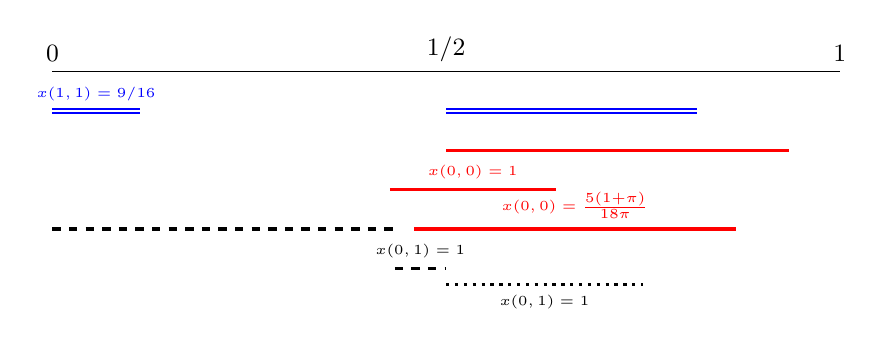
\begin{tikzpicture}
	   %\node[above] (a) at (10/9,0) {\small $1/9$};
	   %\node[above] (b) at (30/11,0) {\small $3/11$};
	   %\node[above] (c) at (90/11,0) {\small $9/11$};
	   \node[above] (d) at (5,0) {\small $1/2$};
	   %\node[above=1cm] (e) at (4.286,0) {\small $3/7$};
	   %\node[above] (f) at (6.393,0) {\small $39/61$};
	   %\node[above=0.5cm] (g) at (4.595,0) {\small $17/37$};
	   %\node[above] (d) at (8.685,0) {\small $251/289$};

	   \draw[above] (0,0) node[above]{\small $0$} -- (10,0) node[above]{\small $1$} ;
	   \draw[thick, style= double, blue] (0,-0.5)--(10/9,-0.5) node[above,midway]{\tiny $x(1,1)=9/16$};
	   \draw[thick, style= double, blue] (5,-0.5)--(90/11,-0.5) ;
	   %Only C1 communicates
	   \draw[very thick, red] (5,-1)--(290/31,-1);
	   \draw[very thick, red] (30/7,-1.5)--(390/61,-1.5) node[above,midway]{\tiny $x(0,0)=1$};
	   \draw[very thick, red] (170/37,-2)--(2510/289,-2) node[above,midway]{\tiny $x(0,0)=\frac{5(1+\pi)}{18\pi}$};
	   %all but Dinfty communicate
	   \draw[very thick, dashed,] (0,-2) -- (100/23,-2);
	   \draw[very thick, dashed] (100/23,-2.5) -- (5,-2.5) node[above,midway]{\tiny $x(0,1)=1$};
	   % Only Ck communicate
	   \draw[very thick, dotted] (5,-2.7) -- (7.5,-2.7) node[below,midway]{\tiny $x(0,1)=1$};
	   % Only Ck communicate
		\end{tikzpicture}
		   
		\caption{Compare CT30 (double,blue) - CT50 (red,black,orange)\\
			red: only $C_1$, dashed: $C_1,C_\infty,D_1$, dotted: $C_1,C_\infty$}
		\label{fig:CT30-CT50}
	\end{figure}


\paragraph{Comparing CT30 and F30}
\begin{itemize}
    \item In CT30 and F30, there is communication only by type $C_1$.
    \item If $\pi\leq \frac{3}{11}$, it is more likely that there is communication in F30 than C30 (communication happens there only if $\pi\leq \frac{1}{9}<\frac{3}{11}$.
    \item If $\pi\geq \frac{1}{2}$, there is no communication in F30 but communication in CT30.
\end{itemize}
See Figure \ref{fig:CT30-F30}. Unless otherwise indicates, $x(1,1)=1$ and $x(1,0)=x(0,0)=x(0,1)=0$.

\begin{figure}[h]
\centering
    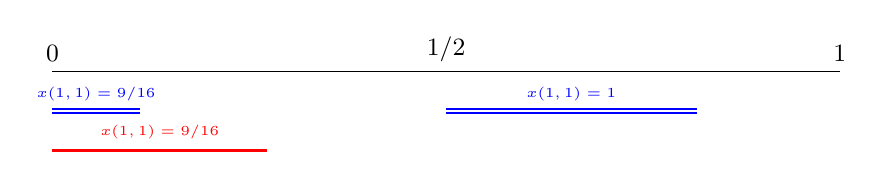
\begin{tikzpicture}
   %\node[above] (a) at (10/9,0) {\small $1/9$};
   %\node[above] (b) at (30/11,0) {\small $3/11$};
   %\node[above] (c) at (90/11,0) {\small $9/11$};
   \node[above] (d) at (5,0) {\small $1/2$};
   \draw[above] (0,0) node[above]{\small $0$} -- (10,0) node[above]{\small $1$} ;
   \draw[thick, style= double, blue] (0,-0.5)--(10/9,-0.5) node[above,midway]{\tiny $x(1,1)=9/16$};
   \draw[thick, style= double, blue] (5,-0.5)--(90/11,-0.5) node[above,midway]{\tiny $x(1,1)=1$};
   \draw[very thick, red] (0,-1)--(30/11,-1) node[above,midway]{\tiny $x(1,1)=9/16$};
    \end{tikzpicture}
       
    \caption{Compare CT30 (double, blue) - F30 (red)}
    \label{fig:CT30-F30}
\end{figure}

\paragraph{Comparing CT50 and FT50}
\begin{itemize}
    \item There is communication equilibria for all $\pi\in\left[0,\frac{29}{31}\right]$ in CT50 but only in the set $\left[\frac{7}{20},\frac{23}{31}\right]\cup \left[\frac{4}{5},\frac{11}{20}\right]$ in F50.
    \item Moreover, in CT50 it is possible for different types to communicate while only type $C_1$ communicates in F50.
    \item In the region $\left[\frac{4}{5},\frac{11}{20}\right]$, type $C_\infty$ cooperates (in the equilibrium state $(0,0)$) with probability one in F50 but with probability less than one in CT50.
\end{itemize}
%
See figure \ref{fig:CT50-F50}. Unless otherwise indicates, $x(1,1)=1$ and $x(1,0)=x(0,0)=x(0,1)=0$.

\begin{figure}[h]
	\centering
		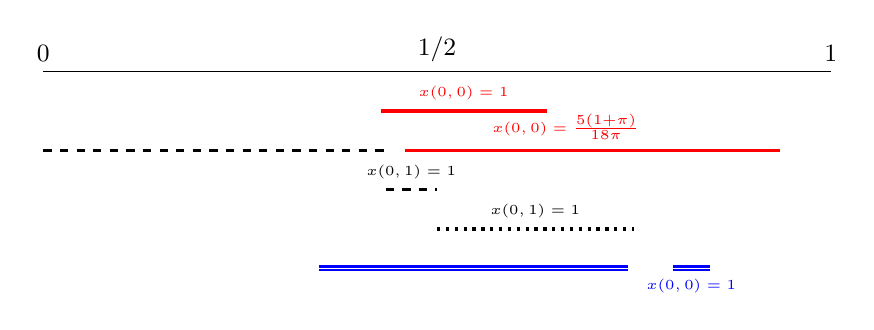
\begin{tikzpicture}
	   %\node[above] (a) at (10/9,0) {\small $1/9$};
	   %\node[above] (b) at (30/11,0) {\small $3/11$};
	   %\node[above] (c) at (90/11,0) {\small $9/11$};
	   \node[above] (d) at (5,0) {\small $1/2$};
	   %\node[above=1cm] (e) at (4.286,0) {\small $3/7$};
	   %\node[above] (f) at (6.393,0) {\small $39/61$};
	   %\node[above=0.5cm] (g) at (4.595,0) {\small $17/37$};
	   %\node[above] (d) at (8.685,0) {\small $251/289$};

	   \draw[above] (0,0) node[above]{\small $0$} -- (10,0) node[above]{\small $1$} ;
	   	   %CT50 Only C1 communicates
	   \draw[very thick, red] (5,-1)--(290/31,-1);
	   \draw[very thick, red] (30/7,-0.5)--(390/61,-0.5) node[above,midway]{\tiny $x(0,0)=1$};
	   \draw[very thick, red] (170/37,-1)--(2510/289,-1) node[above,midway]{\tiny $x(0,0)=\frac{5(1+\pi)}{18\pi}$};
	   %CT50 all but Dinfty communicate<
	   \draw[very thick, dashed] (0,-1) -- (100/23,-1);
	   \draw[very thick, dashed] (100/23,-1.5) -- (5,-1.5) node[above,midway]{\tiny $x(0,1)=1$};
	   % CT50 Only Ck communicate
	   \draw[very thick, dotted] (5,-2) -- (7.5,-2) node[above,midway]{\tiny $x(0,1)=1$};
	   %F50 
	   \draw[thick, style= double, blue] (70/20,-2.5)--(230/31,-2.5) ;
	   \draw[thick, style= double, blue] (8,-2.5)--(110/13,-2.5) node[below,midway]{\tiny $x(0,0)=1$};

		\end{tikzpicture}
		   
		\caption{Compare CT50 (red,dashed,dotted) - F50 (double line, blue)\\
		red: only $C_1$, dashed: $C_1,C_\infty,D_1$, dotted: $C_1,C_\infty$}
		\label{fig:fig:CT30-CT50}
	\end{figure}


	STOPPED HERE (PL)

\section{Theory vs Experimental Results}
Some basic statistics:
\begin{itemize}
	\item $\text{Pr}(Comm|R)$ the probability of sending messages if regime $R\in\{CT,F\}$
	\item $\text{Pr}(C|R)$, $\text{Pr}(D|R)$, the probability that a $C$ or $D$ player communicates in regime $R$.
	\item $x(C|t,R), x(D|t,R)$, the probabilities that a $C$ or $D$ player plays $H$ conditional on state $t$ in regime $R$.
\end{itemize}
In the experiment, $\text{Pr}(Comm|CT30)=75\%$, $\text{Pr}(Comm|CT50)=75\%$, $\text{Pr}(Comm|F30)=17\%$, $\text{Pr}(Comm|F50)=25\%$. By \text{Pr}opositions \ref{prop:CT} and \ref{prop:F}, when $\pi=1/2$ the theoretical probabilities are $\text{Pr}(Comm|CT30)=75\%$, $\text{Pr}(Comm|CT50)=75\%$, $\text{PR}(Comm|F30)=0$, $\text{Pr}(Comm|F50)=25\%$. Hence except for regime $F30$ there is a good fit -- both quantitatively and `qualitatively' -- of the theory with the experimental values. (By Proposition \ref{prop:F}, in regime $F30$ there is communication by $C_1$ if $\pi\leq 3/11$, in which case the probability is equal to $\frac{1-\pi}{2}=\frac{8}{22}=36\%$ but the other probabilities will not match.)

TBC....


\section{Cheap talk - Mixed communication strategies}

\subsection{Only $C$ types communicates}

In this section, we consider mixed communication strategies. We assume that $C_\infty$ types communicate with a probability $\alpha$, while $C_1$ always communicates. Posterior beliefs after communication are $p(C_1|1) = \frac{1-\pi}{1-\pi + \alpha \pi}$, $p(C_\infty|1) = \frac{\alpha \pi}{1-\pi + \alpha \pi}$ and $p(D_k|1) = 0$. Posterior beliefs after no communications are $p(C_1|0) = 0$, $p(C_\infty|0) = \frac{(1-\alpha) \pi}{1+(1-\alpha)\pi}$, $p(D_1|0) = \frac{1-\pi}{1+(1-\alpha)\pi}$ and $p(D_\infty|0) = \frac{\pi}{1+(1-\alpha)\pi}$.

$D_1$ plays $L$ after all communication outcomes. $D_\infty$ plays $L$ if she does not communicate, but plays $H$ after she communicates. $C_\infty$ type plays $H$ after she communicates. We will analyse the behavior of $C_\infty$ type for the remaining states and behavior of $C_1$ type.

When the state is $(0,0)$, then $C_k$ plays $H$ if
\[
\frac{(1-\alpha)\pi}{1+(1-\alpha)\pi}(10+(a-10)x(0,0))+\frac{1}{1+(1-\alpha)\pi}10 \geq \frac{(1-\alpha)\pi}{1+(1-\alpha)\pi}(20+4x(0,0))+\frac{1}{1+(1-\alpha)\pi}20,
\]
or
\[
x(0,0)\geq \frac{10(1+\pi(1-\alpha))}{\pi (1-\alpha)(a-14)}.
\]
$x(0,0)>0$ if $\pi\geq\frac{10}{(1-\alpha)(a-24)}$. When $a=30$, then $x(0,0)$ cannot be positive, so $x(0,0)=0$. When $a=50$, then $x(0,0)>0$ if $\pi \geq \frac{5}{13}\frac{1}{1-\alpha}$ and $\alpha \leq \frac{8}{13}$.

\underline{Case $a=30$.}
In this case, $x(0,0)=0$.

In the state $(0,1)$, $C_k$ type plays $H$ if
\[
\frac{1-\pi}{1-\pi+\alpha\pi}(10+20x(1,0))+\frac{\alpha \pi}{1-\pi+\alpha\pi}30 \geq \frac{1-\pi}{1-\pi+\alpha\pi}(20+4x(1,0))+\frac{\alpha \pi}{1-\pi+\alpha\pi}24,
\]
or
\[
x(1,0)\geq \frac{10-10\pi -6\pi \alpha}{16(1-\pi)}=\frac{5-5\pi -3\pi \alpha}{8(1-\pi)}.
\]

In the state $(1,1)$, $C_1$ type plays $H$ if
\[
\frac{1-\pi}{1-\pi+\alpha\pi}(10+20x(1,1))+\frac{\alpha \pi}{1-\pi+\alpha\pi}30 \geq \frac{1-\pi}{1-\pi+\alpha\pi}(20+4x(1,1))+\frac{\alpha \pi}{1-\pi+\alpha\pi}24-1,
\]
or
\[
x(1,1)\geq \frac{9-9\pi -7\pi \alpha}{16(1-\pi)}.
\]

In the state $(1,0)$, $C_1$ type plays $H$ if
\[
\frac{(1-\alpha)\pi}{1+(1-\alpha)\pi}(10+20x(0,1))+\frac{1}{1+(1-\alpha)\pi}10 \geq \frac{(1-\alpha)\pi}{1+(1-\alpha)\pi}(20+4x(0,1))+\frac{1}{1+(1-\alpha)\pi}20-1,
\]
or
\[
x(0,1)\geq \frac{9(1+\pi(1-\alpha))}{16\pi (1-\alpha)}.
\]
If $\alpha\leq \frac{2}{7}$ then $x(0,1)$ can be positive. If $\alpha\geq \frac{2}{7}$ then $x(0,1)=0$ and $x(0,1)=0$.

If $\alpha\geq \frac{2}{7}$, then $x(0,0)=x(0,1)=x(1,0)=0$. $C_\infty$ type has to be indifferent between communication and no communication.
\[
\frac{\pi}{2}(10+20\alpha)+\frac{1-\pi}{2}(10+20x(1,1))+\frac{1}{2}10=20+2\pi\alpha,
\]
or
\[
x(1,1)=\frac{5+5\pi-8\pi\alpha}{10(1-\pi)}.
\]
This can be true if $x(1,1)=1$, $\alpha=\frac{15\pi-5}{8\pi}$ and $\pi\leq \frac{5}{7}$ or $x(1,1)=\frac{9-9\pi -7\pi \alpha}{16(1-\pi)}$, $\alpha=\frac{90\pi-5}{29\pi}$ and $\pi\leq \frac{5}{61}$.

$C_1$'s incentive to communicate...

$D_1$'s incentive to not communicate...
% section exogenous_cost_of_communication (end)



% section appendix (end)

\bibliographystyle{agsm}
\bibliography{collusion.bib}
\end{document}